\section{Application of Napali in Other domains}\label{sec:application-of-napali-in-other-domains}
Sensor networks are prolific in today's world.
Industrial process and environment monitoring is striving to make the world more efficient and productive.
Medical and Personal sensing is a welcome addition to improving health care and quality of life.
Many of these fields operate in regimes suitable for Napali.
The results of my research provide evidence that Napali is well suited for sensor networks operating in domains with:
\begin{itemize}
    \item Signal to noise ratio of $>1$.
    \item Consensus based event detection.
    \item Two way communication between the device and sink.
\end{itemize}
Any monitoring situation which requires a consensus of multiple devices, with individual devices unable to ascertain the validity of an anomaly is well suited for Napali deployment.
In this section I review potential applications of Napali to several domains intrinsically different from power quality monitoring, while still adhering to the constraints outlined above.

\subsection{Earthquake detection}
Detection of seismic phenomenon is a task well suited for sensor networks.
Single location monitoring is unfeasible, due to a multitude of factors.
Local noise from human activity results in a large number of false positives.
Furthermore, single location monitoring is useless for development of an early warning system.
Earthquake detection relies on prompt detection of P-waves, or pressure waves.
These waves travel faster than their more destructive counterpart: S-waves.
A prompt detection and characterization of a P-wave can provide an early warning of an impending catastrophe.
A large number of sensor networks of varying complexity and sophistication have been deployed in order to monitor geographic areas for seismic activity.\cite{burkett2014shakealert}\cite{zaicenco2012lessons}\cite{klapez2018first}\cite{finazzi2017statistical}

In their paper ``Lessons Learned from Operating an On-site Earthquake Early Warning System"\cite{zaicenco2012lessons} authors Zaicenco and Weir-Jones describe the main challenges for designing and operating an earthquake detection system:
\begin{enumerate}
    \item Unknown direction of a potential seismic event, since sources capable of generating
    the ground motion that exceeds design parameters are spread around the region.
    \item Multiple sources of industrial noise at the site: highway traffic, railroad, fishery, heavy trucks
    driving several meters away from the instrumented area;
    \item Requirement for the system to operate 24/7 in the autonomous mode for several years;
    \item High cost of a potential false alarm, which might result in closing the traffic on the major
    highway.
\end{enumerate}

Their experience comes from operation of borehole sensor arrays located along the highways of British Columbia.
Each sensor array is connected via a fiber drop to the central computer.
Every measurement performed by the sensor array is transmitted to a main processing unit for P-wave analysis.
The triggering algorithm first precomputes a p-wave metric for each sensor, and uses a threshold based algorithm for earthquake detection.
This is a well established system which was able to detect and provide early warning for multiple earthquakes during its operational phase 2009-2011.
The design of this system is very similar to a Naive triggering method for Power Quality monitoring.
All data is funneled to the central sink and processed on site.

The California Integrated Seismic Network is another seismograph sensor network consisting of over 400 high quality borehole sensors.\cite{uhrhammer2011california}
Similarly to the On-site Earthquake Early Warning System, the California Integrated Seismic Network transmits all of the sensor data to the central sink.
The California Integrated Seismic Network is now a part of ShakeAlert, a US-based effort to integrate seismic prediction into actionable intelligence.

Another approach to earthquake monitoring comes from the newly emerged IOT domain.
The cellphone based Earthquake Network \cite{finazzi2017statistical} utilizes smartphone accelerometers in order to detect P-wave propagation throughout the world.
As a part of the Earthquake Network, cellphones which are at rest and plugged into a power source will monitor the internal accelerometer for abnormalities.
If the inertial tensor recorded by the cellphone passes a threshold a message will be transmitted to a central cloudbased sink.
The cloudbased sink in turn uses device location and statistical clustering in order to determine if a P-wave has been detected.
Another IOT sensor network designed for earthquake detection is called Earthcloud.\cite{klapez2018first}
This sensor network utilizes dedicated low cost sensors which communicate via the Internet to the centralized sink.
Similarly to the Earthquake Network, Earthcloud utilizes the number of ``prewarnings"(devices which passed the local threhold) in order to determine if an earthquake is taking place.

Sensor networks described above fall into the two categories described in the previous chapters.
The On-site Earthquake Early Warning System and California Integrated Seismic Network are the Naive approaches with all of the sensor data funneled to the sink.
Earthcloud and Earthquake Network on the other hand are similar to the self-triggered system, with additional statistical analysis performed at the sink.
All three networks maintain two way TCP/IP link between devices and the sink.
With a relatively small number of nodes the On-site Earthquake Early Warning System and California Integrated Seismic Network are able to operate in the Naive mode due to relatively low bandwidth requirements.
On the other hand, Earthquake Network app has 4 million downloads and 75000 active cellphones, and as such is forced to operate in the self triggered mode.

Napali methodology could enhance both of these event detection topologies.
``High quality" earthquake monitoring networks such as California Integrated Seismic Network serve a dual purpose.
First and foremost, they are the nation's early warning system for disaster mitigation.
Second, they are a research and analysis tool used by geophysicist to study earthquake propagation, localization and classification.
Application of Napali to earthquake detection could:
\begin{enumerate}
    \item Reduce the bandwidth requirement for operating a seismic sensor.
    \item Preserve sub-threshold earthquake data for earthquake analysis.
    \item Reject single point anomalies resulting from human activity.
\end{enumerate}
Napali approach could aggregate multiple measurements in order to conserve bandwidth for below threshold events.
If a local threshold is passed, the measurement would be forwarded to the sink immediately in order to provide a timely latency.
If the sink determines that a P-wave has been detected, raw, high resolution data can be requested from the seismic sensor.

Currently IOT approaches are useless for scientific application, since only a ``prewarning" is transmitted to the sink without the high resolution waveform.
With Napali useful high resolution data can be transmitted for later scientific analysis.

\subsection{Lightning Detection}\label{subsec:lightning-detection}
United States National Lightning Detection Network operates over 100 sensors across the United states\cite{cummins1998combined}.
These lightning detectors create a sensor network used to record, detect, localize and  classify lightning strikes.
Data from this network is made available for utilities, National Weather Service and to meteorologists for analysis and study.
Potential uses for this data include cooperation with the Forestry Service, space flight providers, air traffic control, and wind farm operators in order to mitigate lighting risk.\cite{nag2013upgrade}
Lightning detectors are placed in remote areas and communicate via satellite in order to limit interference from anthropogenic sources.
The operational cost of such network can be reduced by placing the lighting detectors in urban centers and other locations they are supposed to protect.
The local man-made noise presents an issue for traditional Self-Triggered operation of such a network, however using Napali, this noise can be filtered out.
Napali has the potential to provide lighting detection at a fraction of the cost of a satellite based system.
Furthermore, sub-threshold data from Napali would allow for better event localization and classification than a conventional Self-Triggered system.

\subsection{Gunshot detection acoustic sensor networks}\label{subsec:gunshot-detection-acustic-sensor-network}
Gunshot detection acoustic sensor networks are generally placed in urban areas.
A multitude of these sensor networks have been proposed in the literature, however the only known operational systems seem to be single
location multi-microphone devices. \cite{bandi2012novel} \cite{khalid2013gunshot}
There are however patents relating to multi-sensor gunshot detection systems, so it is possible that such systems are operated covertly.
All of these systems rely on feature extraction and triggering performed on the device itself, making them Self-Triggered networks.
Napali could enhance the detection capability of these networks through sub-threshold detection as well as on the fly localized false positive rejection.
Once the waveforms from the sensors are acquired, more sophisticated algorithms can be utilized for event localization.

\subsection{Neutrino Physics}\label{subsec:neutrino-physics}
Electron anti-neutrino($\bar{\nu}_e$) is a particularly interesting flavor of a neutrino which interacts with a very specific signature.
An inverse beta decay process is characterized by an $\bar{\nu}_e$ interaction with a proton, resulting a creation of an electron and a positron:
\begin{equation}
    \bar{\nu}_e+p\rightarrow e^++n
\end{equation}
The positron is immediately captured resulting in production of two gammas:
\begin{equation}
    e^+ +e^- \rightarrow \gamma + \gamma
\end{equation}
This is known as the prompt event and it is well characterized in both energy and time.
The neutron will travel through its medium until capture by a nucleus of an atom, resulting in additional gamma release.
This is known as the delayed event, and it will occur within 200us of the initial interaction.
The advantage of the inverse beta decay is that it allows for a well characterised and established detection mechanism for neutrino measurement.
In fact it's the only mechanism we are aware of which uniquely identifies the neutrino.

Many neutrino experiments utilize inverse beta decay as a main physical mechanism.\cite{abe2008precision}\cite{li2016invited}
Unfortunately the chance of the neutrino interaction is extremely small, with many experiments expecting only a few events per day.
In order to maximize data-rate a larger observed volume and a larger number of optical detectors are required.
As such waveform samplers are utilized instead of common ADCs for event capture.

Waveform samplers trade dead time for low power per channel.
Intrinsically, waveform samplers are not ADC in and of itself, instead they are an analog storage medium.
Modern waveform samplers can store $1ms$ or more of analog waveform sampled at $>10Gsps$.
Along with a slow ADC and a triggering system, a waveform sampler allows for extremely fast waveform extraction at the cost of some experiment dead time.
The waveform sampler is filled in a round robin fashion, until the triggering systems determines that an event is occurring.
Once the anomalous condition is identified, the sampler stops, and a slow ADC digitizes all or a portion of the waveform buffer,
The digitized signal is then passed further up the triggering chain.
A Waveform digitizer triggering system is generally a single discriminator per channel built into the the waveform sampler ASIC.
At the lowest layer, the triggering systems count the number of channel discriminator hits and converts them into a triggering metric.
In some cases the geometry of trigger bits is also used in trigger determination.
This layer of the triggering system is commonly referred to as L0.

Tuning the trigger discriminator threshold is a tedious task.
The detectors which the ADCs service are generally optical photon counters sensitive to single photon hits.
However, at this level of sensitivity single photon level noise is prevalent in all optical detector used to date.
This noise, known as dark counts, is usually on the order of a single photon signal, which makes a single channel incapable of discriminating false positives.
Only via the global triggering system can the validity of an event be ascertained.
On the low event rate experiments, the trigger thresholds are tuned to detect a single photon hit, and thus are subject to a lot of noise.\cite{li2016invited}
Furthermore, the physics process of interest is usually buried in the common physical processes which occur at a much higher rate.
This means that the triggering system must discriminate between interesting physics, common physical processes and detector noise.
If the common physical processes are not filtered at the triggering level, the resulting digitization dead time results in an unusable detector.

Napali, in conjunction with additional hardware, could support uninteresting event rejection in low event rate physics experiments utilizing waveform samplers.
Most of the machinery used by Napali is already present.
Each device contains a waveform buffer, and is able to transmit some or all of it to the sink at the triggering systems discretion.
If the single bit discriminator is instead replaced with a 3bit ADC, the Napali statistical triggering system can be used to filter unwanted events without compromising trigger efficiency.
Furthermore, the 3 bit digitizer could be used for both high energy prompt and low energy delayed event without compromising detector dead time.


\section{Future Work}\label{sec:future-work}

There are still several unanswered question with regards to Napali benefits.
From the claims described in Section \ref{intro:section:napali}, the power failure resiliency claim, and the privacy claim remain unproven.
A strategy for evaluating these claims is described in the following sections.

\subsection{Power failure resiliency}\label{subsec:power-failure-resiliancy}

In order to evaluate Napali power failure resiliency, one of two methods must be employed.
The most straightforward way is to add a battery backup the to OPQ Box and perform another evaluation deployment.
The OPQ Box is already designed for battery backup, since the entire device (both the mains and the isolated side), can be powered from a common port.
Furthermore, the expansion header on the OPQ Box is designed to accept as well as deliver power.
A block diagram for the proposed battery backup subsystem is shown in Figure \ref{fig:conc:bat}.
\begin{figure}[ht!]
    \centering
    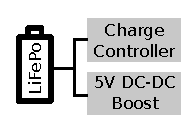
\includegraphics[width=0.5\linewidth]{img/conclusions/battery.pdf}
    \caption{Proposed battery backup subsystem.}
    \label{fig:conc:bat}
\end{figure}
A single cell 14430 LiFePo battery with a capacity of $\approx 1Wh$ could power the OPQ Box for 2 hours in case of a power outage.
A charge controller would keep the battery cell charged during normal operation and the DC-DC boost converter would provide 5V to the OPQ circuitry in case of a mains failure.
This would allow the OPQ Box to record all of the data leading up to the power failure, and if the power outage is shorter than 2 hours capture the moment the power resumes.
A PCB and the battery cell would fit into the existing OPQ Box enclosure with minimum modifications.

Another way to provide power failure resiliency is to add non-volatile memory to the sampler DSP.
Every measurement taken by the DSP would be transferred to the non-volatile memory utilizing it as a circular buffer.
This memory would serve as a black box recording the last measurements taken by the OPQ Box prior to the power failure.
Flash is unsuitable for this due to a relatively small number of write cycles prior to failure, however FRAM devices would be perfect for this application.
2Mb FRAM devices are commonly available on the market, and would allow for an 11s recording window.
The write endurance of $10^{14}$ IOPs results in the device remaining functional for 6000 years.
Data retention of a common FRAM device is 5 years allowing for the data to remain retrievable through the worst of the power outages.
The disadvantage of the non-volatile approach is the device would not be able to capture the moment the power delivery resumes.

\subsection{Privacy Implications}\label{subsec:privacy-implications}
In order to compare the privacy implications of power quality monitoring, and evaluate how Naive and Self-Triggered methods compare, a residential deployment of the OPQ devices must be carried out.
Due to the time constraints such deployment was outside of the scope of this dissertation, however it would be straight forward to carry out.
The main goal of this evaluation would be to empirically measure how much of the end user's activity can be ascertained from the local events which are recorded at their residence.
As such the subjects of these evaluation would deploy the OPQ device at their place of residence and carefully record the timestamp of every electrical appliance they interact with.
From laboratory tests, the OPQ Box was able to detect voltage drops associated with common electrical equipment as shown in Figure \ref{intro:fig:1}.
Since Napali ignores these events, it is expected that it would fare better with respect to end user privacy compared to the Naive and Self-Triggered methods.
Napali does however transmit extracted metrics, however these are aggregated at 1s intervals.
It's unclear how much privacy reduction the Napali methodology would be responsible for, or if the aggregation window length has an impact on privacy as a whole.

\subsection{Grid Hierarchy Clustering on a Larger Scale}\label{subsec:grid-hierarchy-clustering-on-a-larger-scale}
In Section \ref{subsec:clustering-naplai-events}, I described how the grid hierarchy can be extracted from subthreshold information in events captured by Napali.
The advantages of event clustering are significant:
\begin{itemize}
    \item Napali scalability can be linearized by concentrating subthreshold triggering to the cluster boundaries.
    \item Napali can localize the event origin in the grid hierarchy by examining affected clusters.
\end{itemize}

More research is required in order to better understand how to build the hierarchical map of the grid via subthreshold events in an organic automated way.
This can potentially be accomplished by adding an additional layer above the Napali trigger in order to cluster and organize events from new devices added to the network.
Every time a device is added to the network, Napali would start by acquiring its subthreshold data if requested regardless of which cluster the over-threshold event originated from.
As enough data is acquired, the new device will be placed in the appropriate cluster in the triggering hierarchy, and restart normal operations.

\subsection{Artificial Intelligence Integration into the Napali Trigger.}\label{subsec:artafitial-inteligence-integration-into-the-napali-trigger.}
It is unclear if artificial intelligence approaches such as machine learning would fare better than the statistical trigger currently employed in Napali.
While outside the scope of this dissertation, the OPQ deployment provided a large database of metrics and events for training and testing AI constructs.
Furthermore, the Makai triggering service is flexible enough to accommodate any number of triggering algorithms alongside Napali for evaluation, characterization and comparison.
The University of Hawaii power grid and the OPQ network remain a perfect test bed for evaluation of new and emerging power quality detection
techniques through its flexible software architecture from hot-plugable metric extraction, to hot-plugable event detection and capture.

\section{Summary of contributions}\label{sec:conclusions}

In this dissertation I showed that Napali provides a novel architecture that is both a feasible solution to the problem of distributed power quality monitoring and that provides significant benefits over the two standard alternative architectures (all computation/storage at nodes, all computation/storage at the sink).
This was performed via demonstration of validity of the five claims stated in Sections \ref{intro:sec:claim}.
The claims and contributions of this dissertation are summarized in the sections below.

\subsection{Napali minimizes bandwidth usage}\label{subsec:conc:napali-minimizes-bandwidth-usage}
Section \ref{subsec:napali-bandwidth-usage} shows the empirical comparison of Napali, Self-Triggered and Naive triggering system bandwidth consumption in the case of the OPQ deployment.
Naturally, Napali and Self-Triggered methods outperformed the Naive method when it came to bandwidth consumption by a factor of 100x.
By only selecting the anomalous temporal regions for readout, significant bandwidth reduction was observed.
Furthermore, Napali outperformed the Self-Triggered method by further downselection of events to those that impact the power grid.
While the Napali events were larger in size since they constituted raw waveform from multiple devices, they were far fewer in number.
As such Napali was able to achieve a 4x bandwidth reduction over the Self-Triggered method, emerging as a clear winner when it comes to bandwidth consumption.

\subsection{Napali minimizes sink processing requirement}\label{subsec:conc:napali-minimizes-sink-processing-requirement}
Section \ref{subsec:napali-bandwidth-usage} shows the analytical comparison of Napali, Self-Triggered and Naive triggering system bandwidth consumption in the case of the OPQ deployment.
Naturally, the Self-Triggered method fared the worst in this evaluation, since every sample from every device needed to be processed on the sink.
For Napali, overhead in the event detection is minuscule, since the metric comparison and filtering is linear with the number of devices,
resulting in a modest resource consumption increase compared to the Self-Triggered method.
The Self-Triggered method arguably requires no sink resources when it comes to event detection, however the higher levels of event evaluation are impacted by the additional data burden.
For every false positive event that the Self-Triggered framework captures, an additional computational cost is incurred.
While the characterization of this cost is beyond the scope of this work, it was shown that the incurred cost is significant when compared to Napali.

\subsection{Napali mitigates device latency effects}\label{subsec:conc:napali-mitigates-device-latency-effects}
Section \ref{subsec:effects-of-latency-in-the-napali-framework} shows the analytical comparison of Napali, Self-Triggered and Naive triggering system device latency in the case of the OPQ deployment.
Similar to the previous section, no direct comparison between Napali and Self-Triggered event detections methods could be made, since there is no latency impact on the Self-Triggered framework.
The Naive triggering method, on the other hand, required an extremely large waveform buffer in order to accommodate latencies commonly seen by the OPQ Boxes during the University of Hawaii deployment.
Napali was easily able to accommodate latencies of up to an hour by utilizing the waveform buffer in the device itself.
This is significant, since power quality problems could easily result in parts of the network infrastructure such as WIFI access points and routers becoming unavailable.

\subsection{Gridwide monitoring via leaf nodes}\label{subsec:conc:gridwide-monitoring-via-leaf-nodes}
Section \ref{subsec:temporal-locality-triggering-of-the-napali-framework} shows that the edge computing centered approach to power quality monitoring can result in high quality
full and partial gridwide event detection via leaf node monitoring.
The main evaluation of this claim comes from the ground truth measurements delivered via the Utility scale power monitors deployed across the University of Hawaii Campus.
Napali was able to capture every event observed by the meters located higher on the power grid hierarchy apart from localized single phase faults.
The main contribution of this claim is that the power grid can be monitored from regular household voltages without any contribution from the utility company.
This opens a door to an oversight mechanism to monitor Utility due diligence when it comes to the power quality standard.
Furthermore, OPQ was demonstrated to be a reliable system which can be used in conjunction with, but independently from, the Utility for power grid protection.
With the increasing concern about Utility cyber security, an additional independent system is both desired and required.

\subsection{Sub-threshold data acquisition is a viable event detection strategy}\label{subsec:conc:sub-threshold-data-acquisition}
Section \ref{subsec:sub-threshold-data-acquisition} describes the subthreshold detection capability of Napali in the OPQ network.
The main claim of this section is that Napali is able to capture full and partial gridwide events via subthreshold triggering.
Evaluation of this claim was accomplished via ground truth comparison.
While the pool of the ground truth confirmed partial gridwide events which are useful for sub-threshold evaluation is small,
Napali was able to both capture the over threshold and under threshold waveforms associated with each one.
The main contribution of this claim is that the sub-threshold event component is useful in event detection, localization and system scalability.
The consequence of this is shown in Sections \ref{subsec:clustering-naplai-events} and \ref{subsec:event-clustering-evaluation}
where the University power grid was partitioned into the two substations using the subthreshold data, something that would be impossible to do via the Self-Triggered event detection method.

\subsection{Open Power Quality System}\label{subsec:open-power-quality-system}
Another contribution of this work is the Open Power Quality monitoring system.
OPQ Box device has been fully characterized against synthetic data in the laboratory setting as shown in Section \ref{sec:opq-box-characterization.},
and compares favorably to the commercial offerings.
Furthermore the metric extraction algorithms utilized in the OPQ Box have been compared to the Utility meter counterparts in Section \ref{subsubsec:utility-box-comp}, to once again favorable agreement.
The backend infrastructure had 97\% availability during the deployment, brought down only by a power outage and system updates.

\subsection{Napali in other domains}\label{subsec:napali-in-other-domains2}
Applications of Napali in other domains are discussed in Section \ref{sec:application-of-napali-in-other-domains}.
This evaluation shows that Napali usability is not limited to the power quality domain.
Instead Napali's edge-centric sub-threshold detection approach to event detection localization and capture is novel, useful, and can be applied to a variety of important domains.